\documentclass[border=3pt]{standalone}
% Preâmbulo compartilhado pelos diagramas TikZ da aula 12 (Mapeamento por Grade de Ocupação)
\usepackage[T1]{fontenc}
\usepackage[utf8]{inputenc}
\usepackage{lmodern}
\usepackage{amsmath}
\usepackage{xcolor}
\usepackage{tikz}
\usetikzlibrary{arrows.meta,angles,quotes,decorations.pathmorphing,calc,
                positioning,shapes.geometric,shapes.misc,backgrounds,fit,
                math}

% Paleta (mesma dos SVGs originais)
\definecolor{dblue}{HTML}{2A5B8C}
\definecolor{dorange}{HTML}{B3541E}
\definecolor{dgreen}{HTML}{4A7C59}
\definecolor{dred}{HTML}{9C4B4B}
\definecolor{dcream}{HTML}{F4F1EA}
\definecolor{dshade}{HTML}{DDD7C9}

% Função gaussiana (não normalizada por padrão de escala visual)
\pgfmathdeclarefunction{gauss}{3}{%
  \pgfmathparse{1/(#3*sqrt(2*pi))*exp(-((#1-#2)^2)/(2*#3^2))}%
}

% Estilos comuns (prefixo d... para não colidir com chaves internas do pgf)
\tikzset{
  >={Stealth[length=2mm]},
  dguide/.style={gray!55, dashed, line width=0.4pt},
  daxis/.style={gray!60, line width=0.7pt, ->},
  dbody/.style={fill=black!3, draw=black!80, line width=1pt},
  dacc/.style={draw=dblue, line width=1pt},
  dlbl/.style={black!55, font=\small},
  dsub/.style={black!45, font=\footnotesize},
  dstate/.style={circle, draw=black!80, fill=dcream, line width=1pt,
                 minimum size=17mm, font=\large, inner sep=1pt},
  dobs/.style={circle, draw=black!80, fill=dshade, line width=1pt,
               minimum size=14mm, font=\large, inner sep=1pt},
  dbox/.style={rounded corners=2pt, draw=black!80, fill=dcream, line width=1pt,
               align=center, inner sep=6pt},
  dop/.style={circle, draw=black!80, fill=white, line width=1pt,
              minimum size=6mm, inner sep=0pt, font=\small},
  dtrans/.style={->, dblue, line width=1pt},
  dmeas/.style={->, dorange, line width=1pt},
  dcurve/.style={line width=1pt, dblue},
  dcurveb/.style={line width=1.4pt, dorange},
}

\begin{document}
\hyphenpenalty=10000 \exhyphenpenalty=10000 \tolerance=9999 \emergencystretch=3em
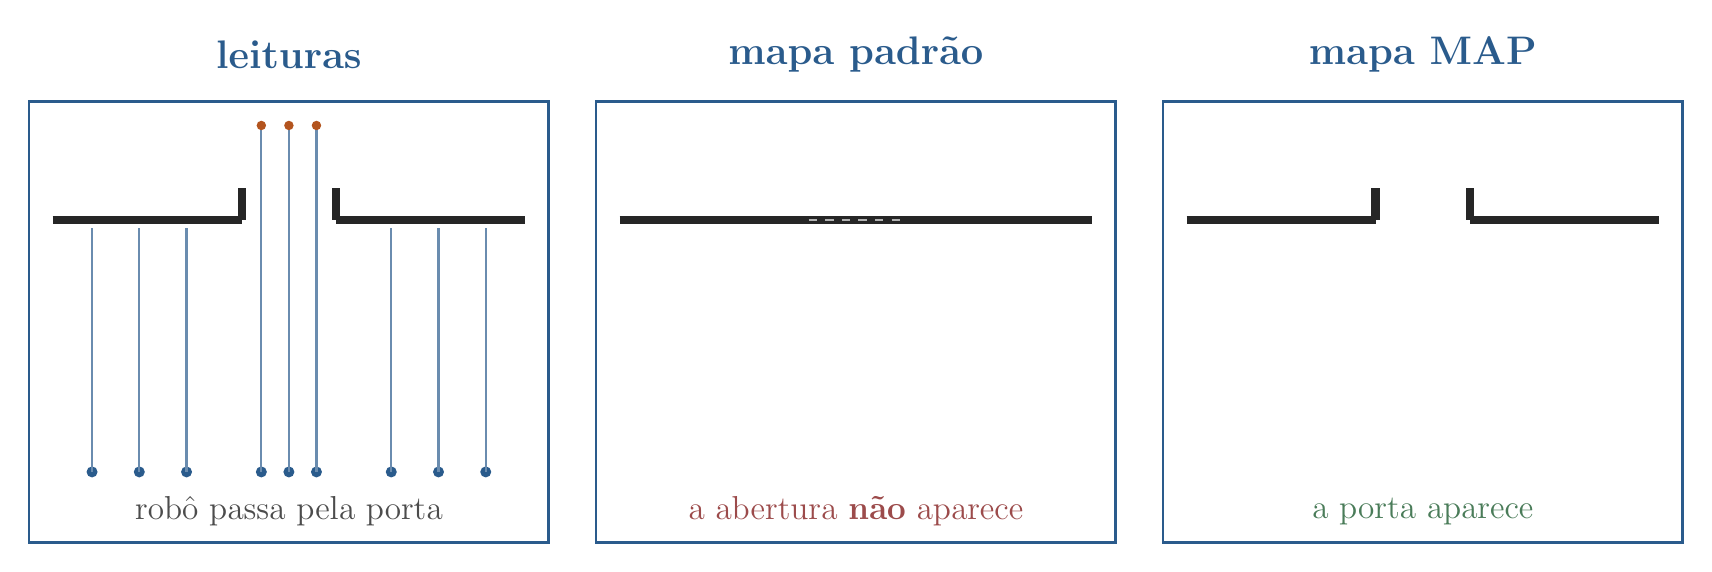
\begin{tikzpicture}[x=1cm,y=1cm]
  \tikzset{wall/.style={line width=3pt, black!85}}
  \foreach \ox/\tt in {0/{leituras}, 7.2/{mapa padrão}, 14.4/{mapa MAP}} {
    \node[font=\Large\bfseries, dblue] at (\ox+3.0,5.3) {\tt};
    \draw[dblue, line width=1pt] (\ox-0.3,-0.9) rectangle (\ox+6.3,4.7);
  }
  % leituras
  \draw[wall] (0,3.2) -- (2.4,3.2); \draw[wall] (3.6,3.2) -- (6,3.2);
  \draw[wall] (2.4,3.2) -- (2.4,3.6); \draw[wall] (3.6,3.2) -- (3.6,3.6);
  \foreach \x in {0.5,1.1,1.7,4.3,4.9,5.5} {\fill[dblue] (\x,0) circle (0.07); \draw[dblue!70, line width=0.8pt] (\x,0) -- (\x,3.1);}
  \foreach \x in {2.65,3.0,3.35} {\fill[dblue] (\x,0) circle (0.07); \draw[dblue!70, line width=0.8pt] (\x,0) -- (\x,4.4); \fill[dorange] (\x,4.4) circle (0.06);}
  \node[font=\large, black!70] at (3.0,-0.5) {robô passa pela porta};
  % mapa padrao: porta fechada
  \draw[wall] (7.2,3.2) -- (13.2,3.2);
  \draw[black!30, dashed, line width=1pt] (9.6,3.2) -- (10.8,3.2);
  \node[font=\large, dred] at (10.2,-0.5) {a abertura \textbf{não} aparece};
  % MAP: porta aberta
  \draw[wall] (14.4,3.2) -- (16.8,3.2); \draw[wall] (18.0,3.2) -- (20.4,3.2);
  \draw[wall] (16.8,3.2) -- (16.8,3.6); \draw[wall] (18.0,3.2) -- (18.0,3.6);
  \node[font=\large, dgreen] at (17.4,-0.5) {a porta aparece};
\end{tikzpicture}
\end{document}
